%% ==============================
\chapter{Dimensionsreduktion}
\label{ch:Dimensionsreduktion}
%% ==============================

Die Dimensionsreduktion hat im Kern das Ziel, einen hochdimensionalen Datensatz auf eine
niedrigdimensionale, sogenannte \newterm{latente} Repräsentation, abzubilden. Dabei soll möglichst
wenig Information über die Daten verloren gehen \parencite[2]{Lee.2007}. Dies ist darin begründet, dass Daten oft nur künstlich hochdimensional, also
\textit{redundant} sind. Die Daten können daher möglicherweise effizienter über eine kleinere Menge
von Merkmalen $y_1,\ldots,y_d$ ausgedrückt werden, als über die ursprüngliche Repräsentation durch
die Merkmale $x_1,\ldots,x_D$ mit $d < D$ und oft $d \ll D$. Hierbei bezeichnet $D$ die
\newterm{extrinsische Dimension} des zugehörigen Ursprungsraumes $\mathcal{X}$ (welcher
üblicherweise dem $\real^D$ entspricht) und $d$ die \newterm{intrinsische Dimension} der Daten. Die
intrinsische Dimension wird teilweise auch als latente Dimension bezeichnet und beschreibt die
minimale Anzahl an Merkmalsvariablen $y_i$, die für die Generierung der Daten benötigt werden \parencite[47]{Lee.2007}. Die intrinsische Dimension kann neben dieser intuitiven Sichtweise auch über
topologische Überlegungen der zugrundeliegenden Verteilung der Daten definiert werden. Diese Idee
wird in \secref{ch:Dimensionsreduktion:MannigfaltigkeitenIntrinsDim} durch das Konzept von
Mannigfaltigkeiten erläutert.

Formell wird die ursprüngliche (hochdimensionale) Repräsentation mit dem $D$-dimensionalen
Zufallsvektor $\rvect{x} = \tr{(x_1, \ldots, x_D)}$ und die latente (niedrigdimensionale)
Repräsentation mit dem $d$-dimensionalen Zufallsvektor $\rvect{y} = \tr{(y_1, \ldots, y_d)}$
gekennzeichnet. Hierbei bezeichnet $\tr{\,(\cdot)\,}$ die Transponierte. Liegt eine konkrete
Stichprobe vor, so werden die einzelnen Stichproben $\vect{x}_i$ mit $i = 1, \ldots,n$ als
Spaltenvektoren in der $n \times D$-Datenmatrix $\mat{X}$ angeordnet. Analog dazu werden die
transformierten (auch: projizierten) Daten in der Matrix $\mat{Y} \in \real^{n \times d}$
angeordnet. Es wird angenommen, dass die Datenmatrix $\mat{X}$ \textit{zentriert} ist. Dies kann
jederzeit durch Subtraktion des Erwartungswertes $\Exp[x_i]$ einer Variable $x_i$ von Spalte $i$
sichergestellt werden.

Nachdem nun die grundlegende Terminologie und das Ziel der Dimensionsreduktion geklärt wurde,
werden im Folgenden einige weitere wichtige Ideen und Konzepte erläutert. Dazu wird in
\secref{ch:Dimensionsreduktion:FluchDerDim} der Fluch der Dimensionalität sowie in
\secref{ch:Dimensionsreduktion:MannigfaltigkeitenIntrinsDim} die Idee von Mannigfaltigkeiten und
der intrinsischen Dimension behandelt. Letztlich wird in \secref{ch:Dimensionsreduktion:Ansaetze}
die Einordnung von Dimensionsreduktionsmethoden besprochen.

\section{Der Fluch der Dimensionalität}
\label{ch:Dimensionsreduktion:FluchDerDim}

Der Term \enquote{Fluch der Dimensionalität} (engl. \textit{Curse of Dimensionality}) wurde von
\textcite{Bellman.1961} im Kontext der Optimierung von Funktionen über hochdimensionale Suchräume
hervorgebracht und ist seitdem zu einem Sammelbegriff für die statistischen Probleme und
Herausforderungen in hochdimensionalen Räumen geworden. Diese Räume weisen unintuitive Phänomene
auf, die in niedrigeren Dimensionen nicht anzutreffen sind. Die zwei Phänomene, die den Begriff
dabei hauptsächlich prägen, sind das \newterm{Phänomen der leeren Räume} und das
\newterm{Konzentrationsphänomen} \parencite[6 -- 9]{Lee.2007}. Diese zwei Phänomene werden im Folgenden kurz erläutert.

Das Konzentrationsphänomen ist auch bekannt als die Konzentration des Maßes (engl.
\textit{concentration of measure}), wobei dahinter eine eigenständige mathematische Theorie steht,
die sich mit Konzentrationsungleichungen befasst \parencite{Ledoux.2001}. Im Kontext des Fluchs der Dimensionalität ist dabei insbesondere die
Konzentration der Normen von Relevanz \parencites[siehe z.B.][]{Kumari.2017}{Verleysen.2005}. Hier kann das Problem des nächsten Nachbarn
betrachtet werden, d.h. zu einem gegebenen Anfragepunkt soll der Punkt mit der kleinsten Distanz
zum Anfragepunkt gefunden werden \parencite[217]{Beyer.1999}. Man stellt fest, dass dies in hochdimensionalen Räumen nicht mehr
effizient gelöst und das Problem sogar bedeutungslos werden kann, wie von \textcite{Beyer.1999}
gezeigt wurde: Die Distanz eines Anfragepunktes zum nächsten Nachbarn stimmt bei steigender
Dimension in Wahrscheinlichkeit mit der Distanz zu dem entferntesten Nachbarn überein. Die Norm
verliert in hohen Dimensionen also an Aussagekraft. \textcite{Aggarwal.2001} untersuchen diesen
Effekt für unterschiedliche Distanzmaße wie der $L_1$-, $L_2$- oder allgemein der $L_p$-Norm und
stellen dabei fest, dass die Aussagekraft einer $L_p$-Norm in höheren Dimensionen für große $p$
schneller abnimmt als z.B. für $p = 2$.

Des Weiteren tritt das Phänomen der leeren Räume auf. Hier stellt man fest, dass hochdimensionale
Räume dünn besetzt sind, da das Volumen im Raum exponentiell mit der Dimension $D$ ansteigt. Möchte
man daher eine Schätzung einer Funktion zu einem gewissen Genauigkeitsgrad durchführen, so steigt
die Anzahl der dazu benötigten Datenpunkte exponentiell mit $D$ an \parencite[6]{Lee.2007}. Dieses Phänomen führt auch zu interessanten Beobachtungen, wie z.B. das
Verhältnis des Volumens einer Hypersphäre und eines Hyperwürfels im $\real^D$ zeigt. Dazu
betrachtet man eine Hypersphäre mit Radius $r$ und den Hyperwürfel, der die Sphäre umschließt, d.h.
die Kantenlänge entspricht dem Durchmesser $2r$ der Sphäre. Das Verhältnis des Volumens dieser
Sphäre zum Volumen des Würfels konvergiert für $D \rightarrow \infty$ gegen Null. Das bedeutet,
dass sich das Volumen in den Ecken konzentriert \parencite[6 -- 7]{Lee.2007} und damit die meisten Punkte weit weg vom Ursprung liegen.

\section{Mannigfaltigkeiten und intrinsische Dimension}
\label{ch:Dimensionsreduktion:MannigfaltigkeitenIntrinsDim}

Wie eingangs besprochen wird bei hochdimensionalen Daten oft von Redundanz oder
Abhängigkeitsstrukturen in den Merkmalen ausgegangen. Eng damit verbunden ist die Idee, dass Daten
auf einer \newterm{Mannigfaltigkeit} (engl. \textit{manifold}) liegen. Auf dieser Idee basierende
Methoden gehören zu einem wichtigen Teilgebiet der Dimensionreduktion: dem Erlernen von
Mannigfaltigkeiten \parencite{Cayton.2005}. Ein Vertreter dieser Methoden ist Locally Linear Embedding, das in
\subsecref{ch:MethodenDerDimRed:statistisch:LLE} noch eingehend behandelt wird. Motiviert werden
diese Ansätze durch die Hypothese, dass reale hochdimensionale Daten in vielen Fällen auf einer in
diesem hochdimensionalen Raum \textit{eingebetteten} Mannigfaltigkeit $\mathcal{M}$ der
Dimensionalität $d$ < $D$ liegen \parencite[vgl.][1]{Cayton.2005}. In diesem Abschnitt wird ein kurzer Überblick über den abstrakten
Begriff einer Mannigfaltigkeit gegeben, wodurch ein geometrischer Bezug der intrinsischen Dimension
hergestellt werden kann.

Eine $d$-dimensionale Mannigfaltigkeit $\mathcal{M}$ ist lokal \textit{homöomorph} zum $\real^d$,
das heißt $\mathcal{M}$ ähnelt \textit{lokal} dem $\real^d$ \parencite[3]{Lee.2011}. Das bedeutet, dass es für jeden Punkt $\vect{z} \in \mathcal{M}$ eine stetige
Abbildung $\varphi: B_\epsilon(\vect{z}) \rightarrow \real^d$ gibt, deren Inverse ebenfalls stetig
ist. Hierbei ist $B_\epsilon(\vect{z})$ ein Ball mit Radius $\epsilon > 0$ um $\vect{z}$. Die
Abbildung $\varphi$ heißt \textit{Karte} und die Gesamtheit aller Karten ergibt den \textit{Atlas}
von $\mathcal{M}$ \parencite[4]{Cayton.2005}. Intuitiv können diese Begriffe besser anhand eines anschaulichen Beispiels
erklärt werden, weshalb in \figref{fig:Torus} ein Torus dargestellt ist. Dieses Objekt ist eine
zweidimensionale Mannigfaltigkeit eingebettet im $\real^3$.
\begin{figure}[ht]
	\centering
	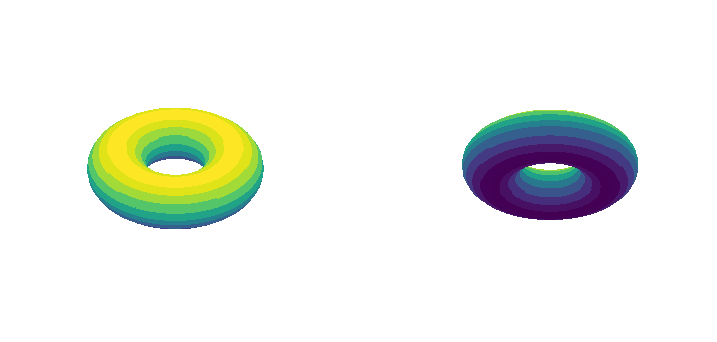
\includegraphics{torus.pdf}
	\caption[Ein Beispiel für eine zweidimensionale Mannigfaltigkeit: ein Torus]{Gezeigt ist ein Beispiel für eine zweidimensionale Mannigfaltigkeit eingebettet im $\real^3$, der sogenannte Torus. Bewegt man sich entlang der Oberfläche des Torus, so erscheint sie lokal flach und ähnelt damit dem $\real^2$. Aus diesem Grund ist der abgebildete Torus eine 2-Mannigfaltigkeit -- trotz der Tatsache, dass das Objekt als Ganzes nicht in einem zweidimensionalen Raum dargestellt werden kann. Eigene Darstellung (angelehnt an \textcite[350]{Hill.2020})}
	\label{fig:Torus}
\end{figure}
Lokal erscheint die Oberfläche des Torus flach, das heißt sie ähnelt dem $\real^2$ und nicht dem $\real^3$, in dem sie eingebettet ist. Die intrinsische Dimension im Kontext der Topologie ist also zwei. Eine Karte kann nun informell wie eine \enquote{Landkarte} eines Teils der Oberfläche des Torus beschrieben werden. Beim Bewegen entlang der Oberfläche kommt es irgendwann zu einem Übergang von zwei Karten. Dieser Übergang von zwei sich
überlappenden Karten wird durch den Homöomorphismus $\varphi$ formalisiert. Betrachtet man alle Karten
von allen Teilen der Oberfläche ergibt dies den Atlas des Torus \parencite[4, 12]{Lee.2012}. Beim Erlernen von Mannigfaltigkeiten geht es nun darum, die latente
Repräsentation $\vect{y}_1, \ldots, \vect{y}_n$ zu finden, für die $\vect{y}_i =
	\varphi(\vect{x}_i)$ gilt. Es wird also angenommen, dass die Punkte $\vect{x}_i$ auf einer
$d$-dimensionalen Mannigfaltigkeit $\mathcal{M}$ liegen, die durch eine einzige Karte $\varphi:
	\mathcal{M} \rightarrow \real^d$ beschrieben werden kann \parencite[4]{Cayton.2005}.

Eine Mannigfaltigkeit kann darüber hinaus noch mit weiteren Eigenschaften versehen werden. Dazu
gehören glatte Mannigfaltigkeiten, auf denen Differentialrechnung möglich ist und ein sogenannter
Tangentialraum definiert werden kann \parencite[50 -- 75]{Lee.2012}. Außerdem kann zwischen zusammenhängenden und nicht-zusammenhängenden
Mannigfaltigkeiten unterschieden werden, wobei letztere aus mehreren nicht-verbundenen
Untermannigfaltigkeiten bestehen. Im restlichen Teil dieser Arbeit wird mit einer Mannigfaltigkeit
Bezug auf eine im $\real^D$ eingebettete $d$-dimensionale Mannigfaltigkeit ohne weitere Annahmen
über die Struktur (glatt, zusammenhängend) genommen. Die intrinsische Dimension von Daten kann also
auch als die topologische Dimension der im $\real^D$ eingebetteten Mannigfaltigkeit $\mathcal{M}$,
auf der die Daten liegen, definiert werden. Auf eine umfassende formale Definition wird an dieser
Stelle jedoch verzichtet. Für eine mathematisch korrekte Definition der hier genannten Begriffe aus
der Topologie wird auf \textcites{Lee.2011}{Lee.2012} verwiesen.

\section{Einordnung der Dimensionsreduktionsmethoden}
\label{ch:Dimensionsreduktion:Ansaetze}
Methoden der Dimensionsreduktion können auf unterschiedliche Weisen in Kategorien eingeteilt werden. Die in dieser Arbeit verwendete Kategorisierung ist in \figref{fig:Kategorisierung} dargestellt und weicht von anderen Taxonomien ab, da der Fokus hier auf dem Vergleich statistischer Methoden und Machine Learning Ansätzen liegt.
% code adapted from https://tex.stackexchange.com/questions/255159/help-on-drawing-a-tree-in-latex?rq=1
\tikzset{
	my node/.style={
			draw=gray,
			inner color=gray!5,
			outer color=gray!10,
			thick,
			minimum width=1cm,
			rounded corners=3,
			text height=1.5ex,
			text depth=0ex,
		}
}
\begin{figure}[h]
	\centering
	\begin{forest}
		for tree={%
		my node,
		l sep+=5pt,
		grow'=south,
		edge={gray, thick},
		parent anchor=south,
		child anchor=north,
		if n children=0{tier=last}{},
		if={isodd(n_children())}{
				for children={
						if={equal(n,(n_children("!u")+1)/2)}{calign with current}{}
					}
			}{}
		}
		[Dimensionsreduktion, s sep=15mm,
		[Machine Learning
					[CAE] [AE]]
			[Statistik
					[LLE] [Kernel PCA] [PCA]]
		]
	\end{forest}
	\caption[Kategorisierung der Dimensionsreduktionsmethoden]{Die hier verwendete Kategorisierung der fünf Methoden.}
	\label{fig:Kategorisierung}
\end{figure}

Statistische Methoden haben eine solide theoretische Fundierung und sind meist etablierte
Algorithmen auf einem jeweiligen Gebiet, wie es zum Beispiel mit der Principal Component Analysis
(\subsecref{ch:MethodenDerDimRed:statistisch:PCA}) der Fall ist. Moderne Machine Learning Methoden
basieren auf neuronalen Netzen und versuchen, aus einer großen Menge an Trainingsdaten eine
Approximation der gesuchten Funktion zu lernen. Autoencoder sind hierfür ein Paradebeispiel und
werden deshalb in \secref{ch:MethodenDerDimRed:modern} eingehend behandelt.

Für einen Überblick und zur besseren Einschätzung wird in diesem Abschnitt ein Auszug der von
\textcite{vanderMaaten.2009} vorgeschlagenen Taxonomie
erläutert.% code adapted from https://tex.stackexchange.com/questions/255159/help-on-drawing-a-tree-in-latex?rq=1
\tikzset{
	my node/.style={
			draw=gray,
			inner color=gray!5,
			outer color=gray!10,
			thick,
			minimum width=1cm,
			rounded corners=3,
			text height=1.5ex,
			text depth=0ex,
		}
}
\begin{figure}[h]
	\centering
	\begin{forest}
		for tree={%
		my node,
		l sep+=5pt,
		grow'=south,
		edge={gray, thick},
		parent anchor=south,
		child anchor=north,
		fit=band,
		if n children=0{tier=last}{},
		if={isodd(n_children())}{
				for children={
						if={equal(n,(n_children("!u")+1)/2)}{calign with current}{}
					}
			}{}
		}
		[Dimensionsreduktion, s sep=15mm,
		[Konvex
			[nicht-vollwertige EWZ [LLE]] [vollwertige EWZ [Kernel PCA] [PCA]]]
		[Nicht-konvex
		[CAE] [AE]]
		]
	\end{forest}
	\caption[Alternative Kategorisierung der Dimensionsreduktionsmethoden]{Ein Auszug aus der Kategorisierung nach \textcite{vanderMaaten.2009}. Eine vollwertige Eigenwertszerlegung (EWZ) zerlegt eine (dichte) Matrix in ihre Eigenwerte und -vektoren. Eine nicht-vollwertige Eigenwertszerlegung meint die Zerlegung einer dünn besetzten Matrix \parencite[3,7]{vanderMaaten.2009}.} \label{fig:KategorisierungMaaten}
\end{figure}

Wie in \figref{fig:KategorisierungMaaten} dargestellt, werden hier die Dimensionsreduktionsmethoden
zunächst in konvexe und nicht-konvexe Methoden eingeordnet. \textbf{Konvexe} Methoden optimieren
eine Zielfunktion, bei der jedes lokale Optimum gleichzeitig das globale Optimum ist. Die
Optimierung ist daher leichter, allerdings sind die möglichen Zielfunktionen auch deutlich
eingeschränkter. Die Lösung dieser Zielfunktionen reduziert sich hier meistens auf ein
Eigenwertproblem, weswegen die konvexen Methoden weiter in Methoden mit einer vollwertigen und
nicht-vollwertigen Eigenwertzerlegung (EWZ) eingegliedert werden können \parencite[3]{vanderMaaten.2009}. \textbf{Nicht-konvexe} Methoden wie der Autoencoder optimieren
nicht-konvexe Zielfunktionen und können damit bei der Optimierung in suboptimalen lokalen
Extrempunkten \enquote{steckenbleiben}. Die Optimierung erfolgt meist mittels des
Gradientenabstiegsverfahrens (engl. \textit{gradient descent}) oder anderer mathematischer
Optimierungsverfahren \parencite[siehe z.B.][]{Guler.2010}.

% \textbf{Distanz-basierte Methoden} versuchen die paarweisen Distanzen in den Daten zu erhalten, womit die zugrundeliegende Struktur erhalten werden soll \parencite[3]{Gracia.2014}. Vertreter dieser Kategorie sind die (klassische) Multidimensionale
% Skalierung \parencites{Kruskal.1964}{Cox.2008}, das Sammon Mapping \addref und die Curvilinear Component Analysis
% \addref. Hierbei muss eine Distanz jedoch nicht die euklidische Distanz zwischen zwei Punkten sein.
% Beispielweise ist die \newterm{geodätische Distanz} als die Distanz entlang der Mannigfaltigkeit
% definiert, auf der die Punkte liegen. Mit dem Hintergrundwissen zu Mannigfaltigkeiten wird
% deutlich, dass euklidische Distanzen vor allem bei nichtlinearen Mannigfaltigkeiten mit einer hohen
% Krümmung irreführend sein können. Die geodätische Distanz wirkt diesem Problem entgegen, ist aber
% nicht immer leicht zu berechnen. Daneben gibt es \textbf{Topologie-erhaltende Methoden}, die
% gezielt die Topologie der Mannigfaltigkeit erhalten wollen und dies durch geometrische Überlegungen
% erzielen \parencite[4]{Gracia.2014}. Zu dieser Kategorie gehört beispielsweise das Locally Linear Embedding
% (\secref{ch:MethodenDerDimRed:statistisch:LLE}), die Self-Organizing Map \parencite{Kohonen.1990} oder die Uniform Manifold Approximation and Projection (UMAP) \parencite{McInnes.2018}.

Neben den in dieser Arbeit vorgestellten Methoden gibt es noch viele weitere
Dimensionsreduktionsmethoden. In der Kategorie der nicht-konvexen Methoden sind dabei das
\textit{Sammon Mapping} \parencite{Sammon.1969} und eine weitere Variante von neuronalen Netzen, den \textit{Self-Organizing
	Maps} \parencite{Kohonen.1990} zu nennen. Eine weitere wichtige konvexe Methode ist das
\textit{Multidimensional Scaling} \parencites{Kruskal.1964}{Cox.2008}, welches in der klassischen Form im Ergebnis sehr ähnlich zur
Principal Component Analysis ist. Des Weiteren sind in dieser Kategorie noch \textit{Isomap} \parencite{Tenenbaum.2000} und Erweiterungen von Locally Linear Embedding wie \textit{Hessian Locally
	Linear Embedding} \parencite{Donoho.2003} oder \textit{Local Tangent Space Alignment} \parencite{Zhang.2002} zu nennen. \textit{Maximum Variance Unfolding} \parencite{Weinberger.2006}, auch bekannt als \textit{Semidefinite Embedding}, erweitert die Kernel
Principal Component Analysis, indem die Kernel-Matrix gelernt wird. Wenn die Dimensionsreduktion
lediglich für die Visualisierung, d.h. für die Reduktion auf zwei oder drei Dimensionen verwendet
wird, sind außerdem \textit{t-distributed Stochastic Neighbor Embedding} \parencite{vanderMaaten.2008} und \textit{Uniform Manifold Approximation and Projection} \parencite{McInnes.2018} vielverwendete Methoden.

Wie zu erkennen ist, gibt es eine große Auswahl an verschiedenen Methoden der Dimensionsreduktion.
Nach dem \newterm{No Free Lunch Theorem} \parencite{Wolpert.1997} gibt es aber keinen \enquote{besten} Algorithmus für jede Situation, weswegen
eine Methode domänenspezifisch ausgewählt werden muss. Zur Reduktion von Speicher- und
Rechenanforderungen und aufgrund des Fluchs der Dimensionalität kann es trotzdem sinnvoll sein,
diesen Aufwand zu betreiben. Mit dem Hintergrundwissen zu wichtigen Konzepten wie der
Mannigfaltigkeit und der intrinsischen Dimension
(\secref{ch:Dimensionsreduktion:MannigfaltigkeitenIntrinsDim}) können im Folgenden die einzelnen
Methoden vorgestellt werden.